\documentclass[12pt,]{article}
\usepackage{lmodern}
\usepackage{amssymb,amsmath}
\usepackage{ifxetex,ifluatex}
\usepackage{fixltx2e} % provides \textsubscript
\ifnum 0\ifxetex 1\fi\ifluatex 1\fi=0 % if pdftex
  \usepackage[T1]{fontenc}
  \usepackage[utf8]{inputenc}
\else % if luatex or xelatex
  \ifxetex
    \usepackage{mathspec}
  \else
    \usepackage{fontspec}
  \fi
  \defaultfontfeatures{Ligatures=TeX,Scale=MatchLowercase}
\fi
% use upquote if available, for straight quotes in verbatim environments
\IfFileExists{upquote.sty}{\usepackage{upquote}}{}
% use microtype if available
\IfFileExists{microtype.sty}{%
\usepackage{microtype}
\UseMicrotypeSet[protrusion]{basicmath} % disable protrusion for tt fonts
}{}
\usepackage[margin=2.54cm]{geometry}
\usepackage{hyperref}
\hypersetup{unicode=true,
            pdftitle={Are the Thermoclines on Wisconsin Lakes Moving Deeper?},
            pdfauthor={Keith Bollt},
            pdfborder={0 0 0},
            breaklinks=true}
\urlstyle{same}  % don't use monospace font for urls
\usepackage{color}
\usepackage{fancyvrb}
\newcommand{\VerbBar}{|}
\newcommand{\VERB}{\Verb[commandchars=\\\{\}]}
\DefineVerbatimEnvironment{Highlighting}{Verbatim}{commandchars=\\\{\}}
% Add ',fontsize=\small' for more characters per line
\usepackage{framed}
\definecolor{shadecolor}{RGB}{248,248,248}
\newenvironment{Shaded}{\begin{snugshade}}{\end{snugshade}}
\newcommand{\KeywordTok}[1]{\textcolor[rgb]{0.13,0.29,0.53}{\textbf{#1}}}
\newcommand{\DataTypeTok}[1]{\textcolor[rgb]{0.13,0.29,0.53}{#1}}
\newcommand{\DecValTok}[1]{\textcolor[rgb]{0.00,0.00,0.81}{#1}}
\newcommand{\BaseNTok}[1]{\textcolor[rgb]{0.00,0.00,0.81}{#1}}
\newcommand{\FloatTok}[1]{\textcolor[rgb]{0.00,0.00,0.81}{#1}}
\newcommand{\ConstantTok}[1]{\textcolor[rgb]{0.00,0.00,0.00}{#1}}
\newcommand{\CharTok}[1]{\textcolor[rgb]{0.31,0.60,0.02}{#1}}
\newcommand{\SpecialCharTok}[1]{\textcolor[rgb]{0.00,0.00,0.00}{#1}}
\newcommand{\StringTok}[1]{\textcolor[rgb]{0.31,0.60,0.02}{#1}}
\newcommand{\VerbatimStringTok}[1]{\textcolor[rgb]{0.31,0.60,0.02}{#1}}
\newcommand{\SpecialStringTok}[1]{\textcolor[rgb]{0.31,0.60,0.02}{#1}}
\newcommand{\ImportTok}[1]{#1}
\newcommand{\CommentTok}[1]{\textcolor[rgb]{0.56,0.35,0.01}{\textit{#1}}}
\newcommand{\DocumentationTok}[1]{\textcolor[rgb]{0.56,0.35,0.01}{\textbf{\textit{#1}}}}
\newcommand{\AnnotationTok}[1]{\textcolor[rgb]{0.56,0.35,0.01}{\textbf{\textit{#1}}}}
\newcommand{\CommentVarTok}[1]{\textcolor[rgb]{0.56,0.35,0.01}{\textbf{\textit{#1}}}}
\newcommand{\OtherTok}[1]{\textcolor[rgb]{0.56,0.35,0.01}{#1}}
\newcommand{\FunctionTok}[1]{\textcolor[rgb]{0.00,0.00,0.00}{#1}}
\newcommand{\VariableTok}[1]{\textcolor[rgb]{0.00,0.00,0.00}{#1}}
\newcommand{\ControlFlowTok}[1]{\textcolor[rgb]{0.13,0.29,0.53}{\textbf{#1}}}
\newcommand{\OperatorTok}[1]{\textcolor[rgb]{0.81,0.36,0.00}{\textbf{#1}}}
\newcommand{\BuiltInTok}[1]{#1}
\newcommand{\ExtensionTok}[1]{#1}
\newcommand{\PreprocessorTok}[1]{\textcolor[rgb]{0.56,0.35,0.01}{\textit{#1}}}
\newcommand{\AttributeTok}[1]{\textcolor[rgb]{0.77,0.63,0.00}{#1}}
\newcommand{\RegionMarkerTok}[1]{#1}
\newcommand{\InformationTok}[1]{\textcolor[rgb]{0.56,0.35,0.01}{\textbf{\textit{#1}}}}
\newcommand{\WarningTok}[1]{\textcolor[rgb]{0.56,0.35,0.01}{\textbf{\textit{#1}}}}
\newcommand{\AlertTok}[1]{\textcolor[rgb]{0.94,0.16,0.16}{#1}}
\newcommand{\ErrorTok}[1]{\textcolor[rgb]{0.64,0.00,0.00}{\textbf{#1}}}
\newcommand{\NormalTok}[1]{#1}
\usepackage{longtable,booktabs}
\usepackage{graphicx,grffile}
\makeatletter
\def\maxwidth{\ifdim\Gin@nat@width>\linewidth\linewidth\else\Gin@nat@width\fi}
\def\maxheight{\ifdim\Gin@nat@height>\textheight\textheight\else\Gin@nat@height\fi}
\makeatother
% Scale images if necessary, so that they will not overflow the page
% margins by default, and it is still possible to overwrite the defaults
% using explicit options in \includegraphics[width, height, ...]{}
\setkeys{Gin}{width=\maxwidth,height=\maxheight,keepaspectratio}
\IfFileExists{parskip.sty}{%
\usepackage{parskip}
}{% else
\setlength{\parindent}{0pt}
\setlength{\parskip}{6pt plus 2pt minus 1pt}
}
\setlength{\emergencystretch}{3em}  % prevent overfull lines
\providecommand{\tightlist}{%
  \setlength{\itemsep}{0pt}\setlength{\parskip}{0pt}}
\setcounter{secnumdepth}{5}
% Redefines (sub)paragraphs to behave more like sections
\ifx\paragraph\undefined\else
\let\oldparagraph\paragraph
\renewcommand{\paragraph}[1]{\oldparagraph{#1}\mbox{}}
\fi
\ifx\subparagraph\undefined\else
\let\oldsubparagraph\subparagraph
\renewcommand{\subparagraph}[1]{\oldsubparagraph{#1}\mbox{}}
\fi

%%% Use protect on footnotes to avoid problems with footnotes in titles
\let\rmarkdownfootnote\footnote%
\def\footnote{\protect\rmarkdownfootnote}

%%% Change title format to be more compact
\usepackage{titling}

% Create subtitle command for use in maketitle
\newcommand{\subtitle}[1]{
  \posttitle{
    \begin{center}\large#1\end{center}
    }
}

\setlength{\droptitle}{-2em}

  \title{Are the Thermoclines on Wisconsin Lakes Moving Deeper?}
    \pretitle{\vspace{\droptitle}\centering\huge}
  \posttitle{\par}
  \subtitle{\url{https://github.com/keithbollt/ENV872BadgerThermoclines.git}}
  \author{Keith Bollt}
    \preauthor{\centering\large\emph}
  \postauthor{\par}
    \date{}
    \predate{}\postdate{}
  

\begin{document}
\maketitle
\begin{abstract}
For this project, I was interested in determining if thermoclines in
five Wisconsin lakes are trending deeper over time, possibly due to
climate change. I looked at physical and chemical data from the NTLR
dataset, specifically temperature and dissolved oxygen levels at 7
meters depth between June 20 and September 21 from every year data was
available between 1984 and 2016. Initial data visualization did not
promise significant trends that would point to climate change. I ran
four total tests on the dataset: a repeated measures ANOVA on the
combined dataset for both variables, and a seasonal Mann Kendall on each
of the five lakes for both variables. I found that there was not a
significant trend in temperature or oxygen on the five lakes as a whole,
and that no individual lake exhibited both a significant increase in
temperature and a significant decrease in dissolved oxygen at 7 meters
depth. In my conclusion, I discuss that for incremental climate change,
the thermocline may not move because it is a result of a lake's relative
physical conditions. Further tests would likely reveal that the
thermocline is steeper.
\end{abstract}

\newpage
*

*Table of Contents**

\begin{longtable}[]{@{}ll@{}}
\toprule
Page Number & Section\tabularnewline
\midrule
\endhead
5 & Setting Up RStudio for Analysis\tabularnewline
7 & Research Question and Rationale\tabularnewline
8 & Dataset Information\tabularnewline
10 & Exploratary Data Analysis and Wrangling\tabularnewline
11 & Analysis\tabularnewline
25 & Discussion\tabularnewline
26 & Appendix: Project README File\tabularnewline
\bottomrule
\end{longtable}

\newpage

\listoftables 

\begin{longtable}[]{@{}ll@{}}
\toprule
Page Number & Table\tabularnewline
\midrule
\endhead
8 & Table 1: Table Summarizing Project Data Structure\tabularnewline
17 & Table 2: Summary of ANOVA Results\tabularnewline
22 & Table 3: Summary of Seasonal Mann Kendall Results\tabularnewline
\bottomrule
\end{longtable}

\newpage

\listoffigures 

\begin{longtable}[]{@{}ll@{}}
\toprule
Page Number & Figure\tabularnewline
\midrule
\endhead
13 & Figure 1: Temperature Distribution at 7 Meters\tabularnewline
13 & Figure 2: ``Temperature versus Dissolved Oxygen''\tabularnewline
14 & Figure 3: ``Paul Lake Temperature Over Time''\tabularnewline
14 & Figure 4: ``Paul Lake Dissolved Oxygen Over Time''\tabularnewline
18 & Figure 5: ``Temperature at 7m of All Lakes Over
Time''\tabularnewline
18 & Figure 6: ``Dissolved Oxygen at 7m of All Lakes Over
Time''\tabularnewline
23 & Figure 7: ``Dissolved Oxygen Over Time in Each
Lake''\tabularnewline
24 & Figure 8: ``Temperature Over Time in Each Lake''\tabularnewline
\bottomrule
\end{longtable}

\newpage

\textbf{Setting Up RStudio for Analysis}

\begin{Shaded}
\begin{Highlighting}[]
\CommentTok{#Setting up session and loading all packages I think I might need}
\KeywordTok{getwd}\NormalTok{()}
\end{Highlighting}
\end{Shaded}

\begin{verbatim}
## [1] "V:/ENV872BadgerThermoclines"
\end{verbatim}

\begin{Shaded}
\begin{Highlighting}[]
\KeywordTok{library}\NormalTok{(tidyverse)}
\end{Highlighting}
\end{Shaded}

\begin{verbatim}
## -- Attaching packages --------------------------------------------------------------------------------- tidyverse 1.2.1 --
\end{verbatim}

\begin{verbatim}
## v ggplot2 3.1.0     v purrr   0.2.5
## v tibble  1.4.2     v dplyr   0.7.8
## v tidyr   0.8.2     v stringr 1.3.1
## v readr   1.3.1     v forcats 0.3.0
\end{verbatim}

\begin{verbatim}
## -- Conflicts ------------------------------------------------------------------------------------ tidyverse_conflicts() --
## x dplyr::filter() masks stats::filter()
## x dplyr::lag()    masks stats::lag()
\end{verbatim}

\begin{Shaded}
\begin{Highlighting}[]
\KeywordTok{library}\NormalTok{(lubridate)}
\end{Highlighting}
\end{Shaded}

\begin{verbatim}
## 
## Attaching package: 'lubridate'
\end{verbatim}

\begin{verbatim}
## The following object is masked from 'package:base':
## 
##     date
\end{verbatim}

\begin{Shaded}
\begin{Highlighting}[]
\KeywordTok{library}\NormalTok{(ggplot2)}
\KeywordTok{library}\NormalTok{(multcompView)}
\KeywordTok{library}\NormalTok{(nlme)}
\end{Highlighting}
\end{Shaded}

\begin{verbatim}
## 
## Attaching package: 'nlme'
\end{verbatim}

\begin{verbatim}
## The following object is masked from 'package:dplyr':
## 
##     collapse
\end{verbatim}

\begin{Shaded}
\begin{Highlighting}[]
\KeywordTok{library}\NormalTok{(lsmeans)}
\end{Highlighting}
\end{Shaded}

\begin{verbatim}
## Loading required package: emmeans
\end{verbatim}

\begin{verbatim}
## The 'lsmeans' package is now basically a front end for 'emmeans'.
## Users are encouraged to switch the rest of the way.
## See help('transition') for more information, including how to
## convert old 'lsmeans' objects and scripts to work with 'emmeans'.
\end{verbatim}

\begin{Shaded}
\begin{Highlighting}[]
\CommentTok{#install.packages("trend")}
\KeywordTok{library}\NormalTok{(trend)}

\CommentTok{#setting a theme for plots}
\NormalTok{mytheme <-}\StringTok{ }\KeywordTok{theme_classic}\NormalTok{(}\DataTypeTok{base_size =} \FloatTok{12.2696}\NormalTok{)}\OperatorTok{+}
\StringTok{  }\KeywordTok{theme}\NormalTok{(}\DataTypeTok{axis.text =} \KeywordTok{element_text}\NormalTok{(}\DataTypeTok{color =} \StringTok{"Blue"}\NormalTok{),}
  \DataTypeTok{legend.position =} \StringTok{"top"}\NormalTok{)}
\NormalTok{  plot.title =}\StringTok{ }\KeywordTok{element_text}\NormalTok{(}\DataTypeTok{hjust =} \FloatTok{0.5}\NormalTok{)}
\KeywordTok{theme_set}\NormalTok{(mytheme)}
\end{Highlighting}
\end{Shaded}

\begin{Shaded}
\begin{Highlighting}[]
\CommentTok{#Reading in the raw lake dataset}
\NormalTok{NTLR_raw <-}\StringTok{ }
\StringTok{  }\KeywordTok{read.csv}\NormalTok{(}\StringTok{"V:/ENV_872_Project_Directory/Data/Raw/NTL-LTER_Lake_ChemistryPhysics_Raw.csv"}\NormalTok{)}
\KeywordTok{View}\NormalTok{(NTLR_raw)}

\CommentTok{#Changing the date column to read as a date}
\KeywordTok{class}\NormalTok{(NTLR_raw}\OperatorTok{$}\NormalTok{sampledate)}
\NormalTok{NTLR_raw}\OperatorTok{$}\NormalTok{sampledate <-}\StringTok{ }\KeywordTok{as.Date}\NormalTok{(NTLR_raw}\OperatorTok{$}\NormalTok{sampledate, }\DataTypeTok{format=}\StringTok{"%m/%d/%y"}\NormalTok{)}
\KeywordTok{class}\NormalTok{(NTLR_raw}\OperatorTok{$}\NormalTok{sampledate)}
\end{Highlighting}
\end{Shaded}

\newpage
*

*Research Question and Rationale**

The crux of this project is to determine if the thermoclines on each of
the 9 Wisconsin lakes in the NTL-LTER chemistry and physics dataset have
moved over the course of the 33 years of data between 1984 and 2016. I
am interested in this question because as a flyfisherman, I have an
interest in coldwater fisheries that rely on thermoclines to survive the
summer weather. Perhaps climate change is affecting where the
thermocline sets up, and therefore shrinking the available summer
habitat of trout.

In order to determine whether thermoclines on these lakes are moving
deeper in the water column, I need to set a benchmark definition for a
thermocline. It looks like there is not enough temporal resolution to
measure close-to-continuous change in thermocline depth over the course
of a given season. Likewise, there is not enough close-to-continous
depth measurements taken at each lake, nor is there consistant data
taken below 10 meters of depth. As such, I will compare what is
occurring at a constant depth near the expected thermocline location at
each lake over time. The depth that I chose for the purpose of this
study is 7 meters. 7 meters, I know from my experience as a fisherman,
is on the shallow end of where a thermocline sets up in a northern US
lake. In addition, there is enough temporal resolution at seven meters
to perform statistical analysis on five of the lakes in the raw dataset.
Therefore, evaluating what is happening at 7m depth in each lake will
give a good idea what sorts of conditions trout are dealing with in
these lakes in the summmer. I know from data visualization that did not
make my final report that there is much more variation by year at 7
meters depth than at, say, 10 meters depth. This indicates that 7 meters
is indeed a pretty good estimation of thermocline location for these
lakes. Looking for change at 7 meters should give me a good picture of
whether the thermocline in these lakes is changing over time.

I will look at two indicators of thermocline establishment at 7 meters:
temperature and dissolved oxygen content. I would expect water at or
below the thermocline to have low temperatures and hypoxic conditions
(low oxygen levels). If the thermoclines on these lakes are trending
deeper over the course of my dataset, I would expect most of the lakes
to show increasing temperatures and increasing dissolved oxygen levels
at a 7 meter depth.

My research question, then, is as follows:

How have temperature and oxygen conditions changed at 7 meters depth in
a series of Wisconsin Lakes? Is climate change affecting where the
thermocline sets up in these lakes?

\newpage
*

*Dataset Information**

The dataset used for this project was prepared for Environmental Data
Analytics (ENV 872L) at Duke University's Nicholas School of the
Environment for the spring 2019 semester by Professor Kateri Salk.The
dataset contains physical and chemical data from nine lakes in
Wisconsin. The data was collected between 1984 and 2016 as part of the
NSF-funded North Temperate Lakes Long Term Ecological Research Station.
The data is measured at a station in the middle of each of the nine
lakes. Generally, the data was collected in the morning. The data is
taken at increments, and most data is taken at or below ten meters
depth. The temporal resolution varies across lakes. Some lakes only have
a few years of data, while others have ample data from most or all
years.Data was collected at irregular 1 to 7 day increments from May
through August of each year. The data was taken during periods of no ice
on the lake. This means that there is little data during the winter
months. While there are several different measurements taken at these
lakes, the two variables that the thermocline study focuses on are
dissolved oxygen and temperature. A table summarizing the data structure
of this project is provided at the end of this section. Data collection
techniques used during the period 1984-1990 were described by Carpenter
and Kitchell (1993) and data collection techniques for 1991-1997 were
described by Carpenter et al. (2001).

Carpenter, S.R. and J.F. Kitchell (eds.). 1993. The Trophic Cascade in
Lakes. Cambridge University Press, Cambridge, England.

Carpenter, S.R., J.J. Cole, J.R. Hodgson, J.F. Kitchell, M.L. Pace,D.
Bade, K.L. Cottingham, T.E. Essington, J.N. Houser and D.E. Schindler.
2001. Trophic cascades, nutrients and lake productivity: whole-lake
experiments. Ecological Monographs 71: 163-186."

Table 1: Table Summarizing Project Data Structure:

\begin{longtable}[]{@{}ll@{}}
\toprule
\begin{minipage}[b]{0.33\columnwidth}\raggedright\strut
Element\strut
\end{minipage} & \begin{minipage}[b]{0.61\columnwidth}\raggedright\strut
Details\strut
\end{minipage}\tabularnewline
\midrule
\endhead
\begin{minipage}[t]{0.33\columnwidth}\raggedright\strut
Data Source\strut
\end{minipage} & \begin{minipage}[t]{0.61\columnwidth}\raggedright\strut
North Temperate Lakes Long Term Ecological Research Station\strut
\end{minipage}\tabularnewline
\begin{minipage}[t]{0.33\columnwidth}\raggedright\strut
Data Scraper\strut
\end{minipage} & \begin{minipage}[t]{0.61\columnwidth}\raggedright\strut
Professor Kateri Salk, PhD, Duke University;
\href{mailto:kateri.salk@duke.edu}{\nolinkurl{kateri.salk@duke.edu}}\strut
\end{minipage}\tabularnewline
\begin{minipage}[t]{0.33\columnwidth}\raggedright\strut
More Information about Data\strut
\end{minipage} & \begin{minipage}[t]{0.61\columnwidth}\raggedright\strut
\url{https://lter.limnology.wisc.edu/about/overview}\strut
\end{minipage}\tabularnewline
\begin{minipage}[t]{0.33\columnwidth}\raggedright\strut
Link to Access Data\strut
\end{minipage} & \begin{minipage}[t]{0.61\columnwidth}\raggedright\strut
\url{https://lter.limnology.wisc.edu/data}\strut
\end{minipage}\tabularnewline
\begin{minipage}[t]{0.33\columnwidth}\raggedright\strut
Dimensions of Raw Dataset\strut
\end{minipage} & \begin{minipage}[t]{0.61\columnwidth}\raggedright\strut
38,614 Observations of 11 variables over nine lakes\strut
\end{minipage}\tabularnewline
\begin{minipage}[t]{0.33\columnwidth}\raggedright\strut
Dimensions of Processed Dataset\strut
\end{minipage} & \begin{minipage}[t]{0.61\columnwidth}\raggedright\strut
1,116 Observations of 8 variables over five lakes\strut
\end{minipage}\tabularnewline
\begin{minipage}[t]{0.33\columnwidth}\raggedright\strut
Variables in Processed Dataset\strut
\end{minipage} & \begin{minipage}[t]{0.61\columnwidth}\raggedright\strut
lakename (lake name), year4 (year), daynum (Julian day number),
sampledate (date of observation), depth of observation (in meters),
temperature\_C (lake temperature in degrees Celsius), dissolved Oxygen
(percent dissolved Oxygen), Week (numbered week of the year)\strut
\end{minipage}\tabularnewline
\begin{minipage}[t]{0.33\columnwidth}\raggedright\strut
Temporal Resolution of Processed Dataset\strut
\end{minipage} & \begin{minipage}[t]{0.61\columnwidth}\raggedright\strut
Irregular collection intervals from June 20 to September 21,
1984-2016\strut
\end{minipage}\tabularnewline
\bottomrule
\end{longtable}

\newpage  

\textbf{Exploratory Data Analysis Wrangling}

In order to answer my research question, I need to wrangle my data to
only include the data relevant to my study and to organize it by lake. I
only want data during the summer months (June 20 through September 21)
because this is the time of year when the thermocline is the steepest
and coldwater fish are the most thermally stressed. I also only want
data collected at a 7 meter depth. My first step is to filter my raw
data to generate a dataset for each of the nine lakes.This data summary
gives me the names of the nine lakes.

\begin{Shaded}
\begin{Highlighting}[]
\KeywordTok{unique}\NormalTok{(NTLR_raw}\OperatorTok{$}\NormalTok{lakename)  }
\NormalTok{Paullake_raw <-}\StringTok{ }\NormalTok{NTLR_raw }\OperatorTok
\StringTok{  }\KeywordTok{filter}\NormalTok{(lakename }\OperatorTok{==}\StringTok{ "Paul Lake"}\NormalTok{)}
\NormalTok{Peterlake_raw <-}\StringTok{ }\NormalTok{NTLR_raw }\OperatorTok
\StringTok{  }\KeywordTok{filter}\NormalTok{(lakename }\OperatorTok{==}\StringTok{ "Peter Lake"}\NormalTok{)}
\NormalTok{Tuesdaylake_raw <-}\StringTok{ }\NormalTok{NTLR_raw }\OperatorTok
\StringTok{  }\KeywordTok{filter}\NormalTok{(lakename }\OperatorTok{==}\StringTok{ "Tuesday Lake"}\NormalTok{)}
\NormalTok{Eastlonglake_raw <-}\StringTok{ }\NormalTok{NTLR_raw }\OperatorTok
\StringTok{  }\KeywordTok{filter}\NormalTok{(lakename }\OperatorTok{==}\StringTok{ "East Long Lake"}\NormalTok{)}
\NormalTok{Westlonglake_raw <-}\StringTok{ }\NormalTok{NTLR_raw }\OperatorTok
\StringTok{  }\KeywordTok{filter}\NormalTok{(lakename }\OperatorTok{==}\StringTok{ "West Long Lake"}\NormalTok{)}
\NormalTok{Centrallonglake_raw <-}\StringTok{ }\NormalTok{NTLR_raw }\OperatorTok
\StringTok{  }\KeywordTok{filter}\NormalTok{(lakename }\OperatorTok{==}\StringTok{ "Central Long Lake"}\NormalTok{)}
\NormalTok{Hummingbirdlake_raw <-}\StringTok{ }\NormalTok{NTLR_raw }\OperatorTok
\StringTok{  }\KeywordTok{filter}\NormalTok{(lakename }\OperatorTok{==}\StringTok{ "Hummingbird Lake"}\NormalTok{)}
\NormalTok{Cramptonlake_raw <-}\StringTok{ }\NormalTok{NTLR_raw }\OperatorTok
\StringTok{  }\KeywordTok{filter}\NormalTok{(lakename }\OperatorTok{==}\StringTok{ "Crampton Lake"}\NormalTok{)}
\NormalTok{Wardlake_raw <-}\StringTok{ }\NormalTok{NTLR_raw }\OperatorTok
\StringTok{  }\KeywordTok{filter}\NormalTok{(lakename }\OperatorTok{==}\StringTok{ "Ward Lake"}\NormalTok{)}
\end{Highlighting}
\end{Shaded}

My next step is to filter my dataset to only include data collected at 7
meters depths between June 20 and September 21. I also checked the
dimensions of my wrangled data to make sure each lake still had enough
datapoints to perform statistical analysis on.

\begin{Shaded}
\begin{Highlighting}[]
\NormalTok{Paullake_processed <-}\StringTok{ }\NormalTok{Paullake_raw }\OperatorTok
\StringTok{  }\KeywordTok{filter}\NormalTok{(depth }\OperatorTok{==}\StringTok{ }\DecValTok{7}\NormalTok{, daynum }\OperatorTok\StringTok{ }\DecValTok{172}\OperatorTok{:}\DecValTok{264}\NormalTok{) }\OperatorTok
\StringTok{  }\KeywordTok{select}\NormalTok{(lakename}\OperatorTok{:}\NormalTok{dissolvedOxygen) }\OperatorTok
\StringTok{  }\KeywordTok{mutate}\NormalTok{(}\DataTypeTok{Week =} \KeywordTok{week}\NormalTok{(sampledate)) }\OperatorTok
\StringTok{  }\KeywordTok{na.exclude}\NormalTok{()}
\KeywordTok{dim}\NormalTok{(Paullake_processed)  }

\NormalTok{Peterlake_processed <-}\StringTok{ }\NormalTok{Peterlake_raw }\OperatorTok
\StringTok{  }\KeywordTok{filter}\NormalTok{(depth }\OperatorTok{==}\StringTok{ }\DecValTok{7}\NormalTok{, daynum }\OperatorTok\StringTok{ }\DecValTok{172}\OperatorTok{:}\DecValTok{264}\NormalTok{)}\OperatorTok
\StringTok{  }\KeywordTok{select}\NormalTok{(lakename}\OperatorTok{:}\NormalTok{dissolvedOxygen) }\OperatorTok
\StringTok{  }\KeywordTok{mutate}\NormalTok{(}\DataTypeTok{Week =} \KeywordTok{week}\NormalTok{(sampledate)) }\OperatorTok
\StringTok{  }\KeywordTok{na.exclude}\NormalTok{()}
\KeywordTok{dim}\NormalTok{(Peterlake_processed) }
\CommentTok{#Enough datapoints to analyse this lake.}

\NormalTok{Tuesdaylake_processed <-}\StringTok{ }\NormalTok{Tuesdaylake_raw }\OperatorTok
\StringTok{  }\KeywordTok{filter}\NormalTok{(depth }\OperatorTok{==}\StringTok{ }\DecValTok{7}\NormalTok{, daynum }\OperatorTok\StringTok{ }\DecValTok{172}\OperatorTok{:}\DecValTok{264}\NormalTok{)}\OperatorTok
\StringTok{  }\KeywordTok{select}\NormalTok{(lakename}\OperatorTok{:}\NormalTok{dissolvedOxygen) }\OperatorTok
\StringTok{  }\KeywordTok{mutate}\NormalTok{(}\DataTypeTok{Week =} \KeywordTok{week}\NormalTok{(sampledate)) }\OperatorTok
\StringTok{  }\KeywordTok{na.exclude}\NormalTok{()}
\KeywordTok{dim}\NormalTok{(Tuesdaylake_processed) }\CommentTok{#Enough datapoints to analyse this lake.}

\NormalTok{Eastlonglake_processed <-}\StringTok{ }\NormalTok{Eastlonglake_raw }\OperatorTok
\StringTok{  }\KeywordTok{filter}\NormalTok{(depth }\OperatorTok{==}\StringTok{ }\DecValTok{7}\NormalTok{, daynum }\OperatorTok\StringTok{ }\DecValTok{172}\OperatorTok{:}\DecValTok{264}\NormalTok{)}\OperatorTok
\StringTok{  }\KeywordTok{select}\NormalTok{(lakename}\OperatorTok{:}\NormalTok{dissolvedOxygen) }\OperatorTok
\StringTok{  }\KeywordTok{mutate}\NormalTok{(}\DataTypeTok{Week =} \KeywordTok{week}\NormalTok{(sampledate)) }\OperatorTok
\StringTok{  }\KeywordTok{na.exclude}\NormalTok{()}
\KeywordTok{dim}\NormalTok{(Eastlonglake_processed) }
\CommentTok{#Enough datapoints to analyse this lake.}

\NormalTok{Westlonglake_processed <-}\StringTok{ }\NormalTok{Westlonglake_raw }\OperatorTok
\StringTok{  }\KeywordTok{filter}\NormalTok{(depth }\OperatorTok{==}\StringTok{ }\DecValTok{7}\NormalTok{, daynum }\OperatorTok\StringTok{ }\DecValTok{172}\OperatorTok{:}\DecValTok{264}\NormalTok{)}\OperatorTok
\StringTok{  }\KeywordTok{select}\NormalTok{(lakename}\OperatorTok{:}\NormalTok{dissolvedOxygen) }\OperatorTok
\StringTok{  }\KeywordTok{mutate}\NormalTok{(}\DataTypeTok{Week =} \KeywordTok{week}\NormalTok{(sampledate)) }\OperatorTok
\StringTok{  }\KeywordTok{na.exclude}\NormalTok{()}
\KeywordTok{dim}\NormalTok{(Westlonglake_processed) }
\CommentTok{#Enough datapoints to analyse this lake.}

\NormalTok{Centrallonglake_processed <-}\StringTok{ }\NormalTok{Centrallonglake_raw }\OperatorTok
\StringTok{  }\KeywordTok{filter}\NormalTok{(depth }\OperatorTok{==}\StringTok{ }\DecValTok{7}\NormalTok{, daynum }\OperatorTok\StringTok{ }\DecValTok{172}\OperatorTok{:}\DecValTok{264}\NormalTok{)}\OperatorTok
\StringTok{  }\KeywordTok{select}\NormalTok{(lakename}\OperatorTok{:}\NormalTok{dissolvedOxygen) }\OperatorTok
\StringTok{  }\KeywordTok{mutate}\NormalTok{(}\DataTypeTok{Week =} \KeywordTok{week}\NormalTok{(sampledate)) }\OperatorTok
\StringTok{  }\KeywordTok{na.exclude}\NormalTok{()  }
\KeywordTok{dim}\NormalTok{(Centrallonglake_processed) }
\CommentTok{#There are 0 data points taken on Central Long Lake below 4 meters. }

\NormalTok{Hummingbirdlake_processed <-}\StringTok{ }\NormalTok{Hummingbirdlake_raw }\OperatorTok
\StringTok{  }\KeywordTok{filter}\NormalTok{(depth }\OperatorTok{==}\StringTok{ }\DecValTok{7}\NormalTok{, daynum }\OperatorTok\StringTok{ }\DecValTok{172}\OperatorTok{:}\DecValTok{264}\NormalTok{)}\OperatorTok
\StringTok{  }\KeywordTok{select}\NormalTok{(lakename}\OperatorTok{:}\NormalTok{dissolvedOxygen) }\OperatorTok
\StringTok{  }\KeywordTok{mutate}\NormalTok{(}\DataTypeTok{Week =} \KeywordTok{week}\NormalTok{(sampledate)) }\OperatorTok
\StringTok{  }\KeywordTok{na.exclude}\NormalTok{()  }
\KeywordTok{dim}\NormalTok{(Hummingbirdlake_processed) }
\CommentTok{#Hummingbird lake only has one datapoint at 7 meters. }

\NormalTok{Cramptonlake_processed <-}\StringTok{ }\NormalTok{Cramptonlake_raw }\OperatorTok
\StringTok{  }\KeywordTok{filter}\NormalTok{(depth }\OperatorTok{==}\StringTok{ }\DecValTok{7}\NormalTok{, daynum }\OperatorTok\StringTok{ }\DecValTok{172}\OperatorTok{:}\DecValTok{264}\NormalTok{)}\OperatorTok
\StringTok{  }\KeywordTok{select}\NormalTok{(lakename}\OperatorTok{:}\NormalTok{dissolvedOxygen) }\OperatorTok
\StringTok{  }\KeywordTok{mutate}\NormalTok{(}\DataTypeTok{Week =} \KeywordTok{week}\NormalTok{(sampledate)) }\OperatorTok
\StringTok{  }\KeywordTok{na.exclude}\NormalTok{()}
\KeywordTok{dim}\NormalTok{(Cramptonlake_processed) }
\CommentTok{#There are only 34 datapoints, not enough datapoints to analyse this lake.}

\NormalTok{Wardlake_processed <-}\StringTok{ }\NormalTok{Wardlake_raw }\OperatorTok
\StringTok{  }\KeywordTok{filter}\NormalTok{(depth }\OperatorTok{==}\StringTok{ }\DecValTok{7}\NormalTok{, daynum }\OperatorTok\StringTok{ }\DecValTok{172}\OperatorTok{:}\DecValTok{264}\NormalTok{)}\OperatorTok
\StringTok{  }\KeywordTok{select}\NormalTok{(lakename}\OperatorTok{:}\NormalTok{dissolvedOxygen) }\OperatorTok
\StringTok{  }\KeywordTok{mutate}\NormalTok{(}\DataTypeTok{Week =} \KeywordTok{week}\NormalTok{(sampledate)) }\OperatorTok
\StringTok{  }\KeywordTok{na.exclude}\NormalTok{() }
\KeywordTok{dim}\NormalTok{(Wardlake_processed) }
\CommentTok{#Ward lake only has 11 datapoints at 7 meters. }
\end{Highlighting}
\end{Shaded}

After deciding on what question I wanted to answer and what data I
wanted to use to answer my question, I unfortunately had to eliminate
four lakes from my analysis. I still have five lakes to perform my
analysis on. I also combined my five processed datasets into one
dataframe for part of my statistical analysis. My first series of
statistical tests will look at the combined dataset and my second series
of statistical tests will look at each lake individually.

\begin{Shaded}
\begin{Highlighting}[]
\NormalTok{NTL_processed <-}\StringTok{ }\KeywordTok{rbind}\NormalTok{(Paullake_processed, Peterlake_processed, }
\NormalTok{                       Tuesdaylake_processed,}
\NormalTok{                      Eastlonglake_processed, Westlonglake_processed)}
\KeywordTok{View}\NormalTok{(NTL_processed)}
\KeywordTok{unique}\NormalTok{(NTL_processed}\OperatorTok{$}\NormalTok{lakename)}
\KeywordTok{dim}\NormalTok{(NTL_processed)}
\KeywordTok{head}\NormalTok{(NTL_processed)}
\end{Highlighting}
\end{Shaded}

Now, I will perform a little data visualization before my data analysis.
I hope to get a feel for the data I am working with, and maybe
anticipate the types of results I will find when I perform statistical
analyses in the next section of this report.

See Figure 1 below, which graphs the temperature data distribution for
each of the five lakes at 7m depth. This figure tells us which lakes are
coldest in the summer.

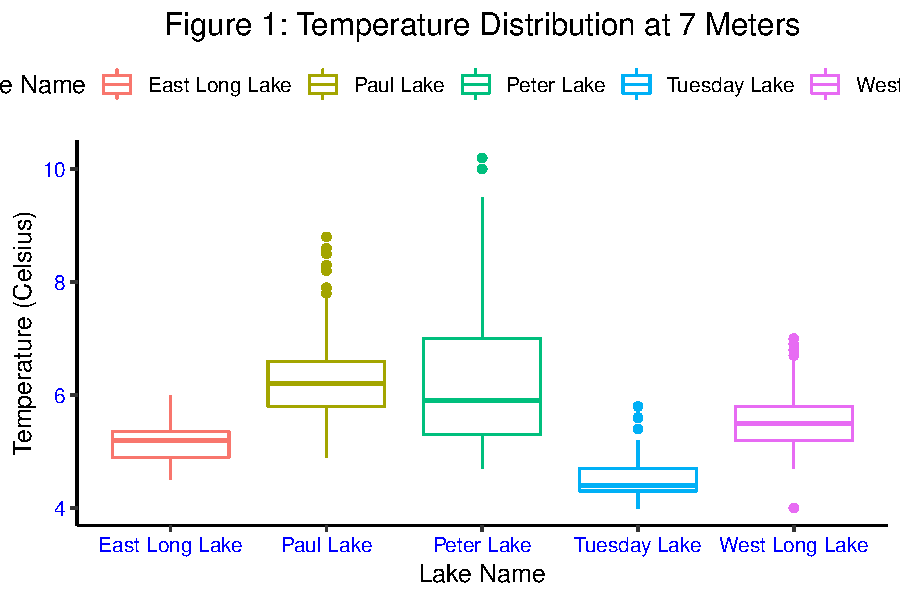
\includegraphics{KBollt_ENV872_FinalProject_files/figure-latex/visualization-1.pdf}

See in Figure 2: ``Temperature versus Dissolved Oxygen'' that there is
no real correlation between temperature and dissolved oxygen at 7 meters
depth across the five lakes.

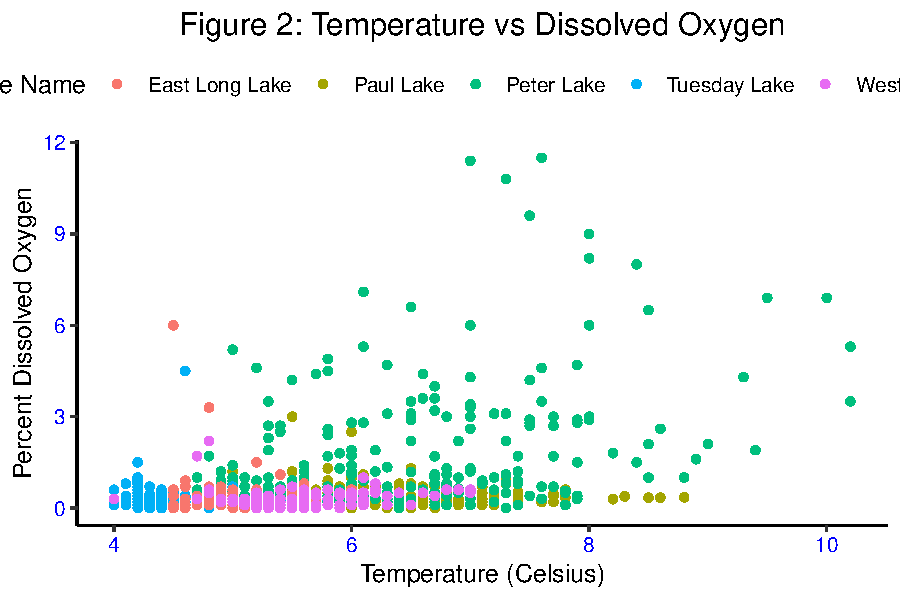
\includegraphics{KBollt_ENV872_FinalProject_files/figure-latex/visualization2-1.pdf}

See in Figure 3: ``Paul Lake Temperature Over Time'' there is not really
much of a trend in temperature in Paul Lake at 7 m depth over time.

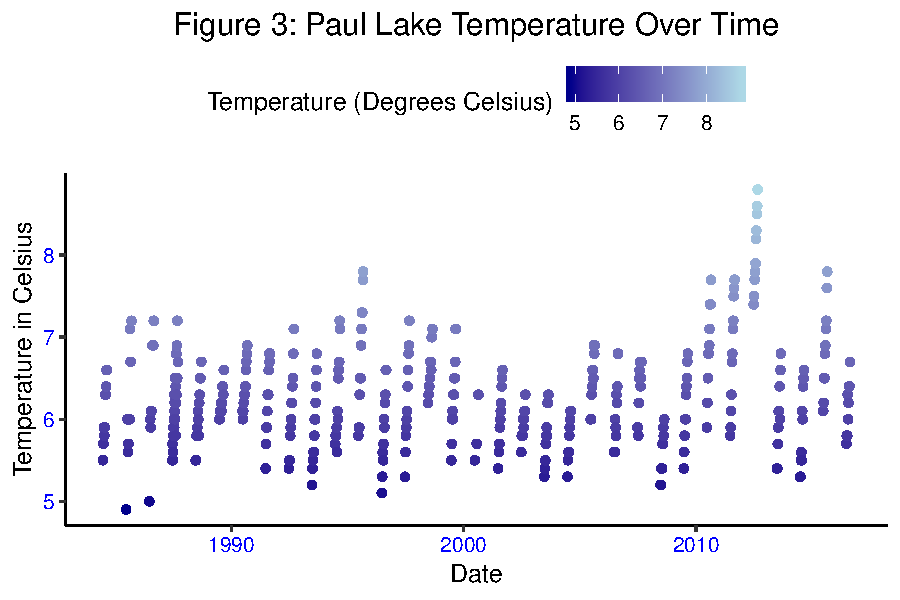
\includegraphics{KBollt_ENV872_FinalProject_files/figure-latex/visualization3-1.pdf}

See in Figure 4: ``Paul Lake Dissolved Oxygen Over Time'' there is not
really much of a trend in dissolved oxygen in Paul Lake at 7 m depth
over time.

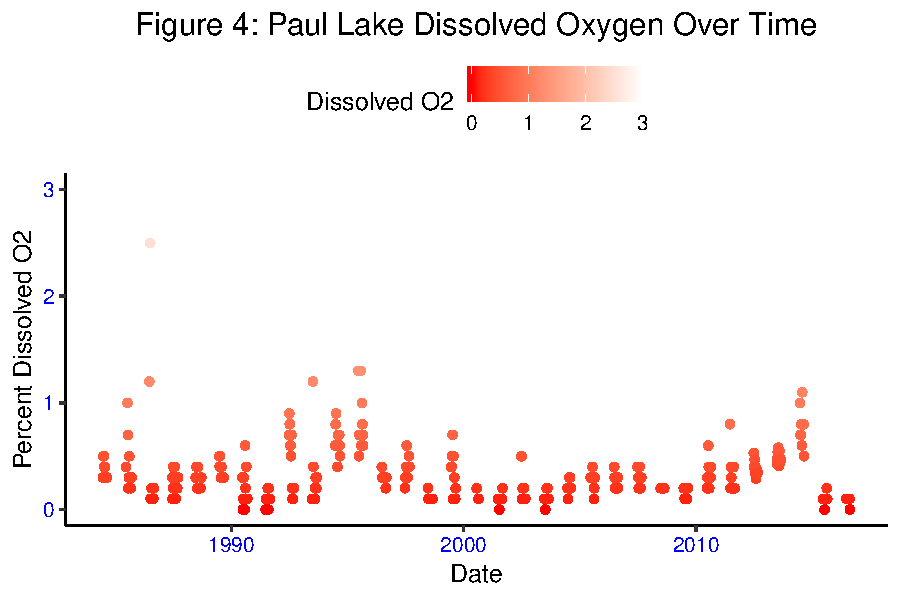
\includegraphics{KBollt_ENV872_FinalProject_files/figure-latex/visualization4-1.pdf}

Overall, my data visualization is not too promising yet. Paul Lake does
not seem to have a trend in either temperature or dissolved oxygen over
time. Likewise, the combined dataset does not appear to have a trend in
temperature over time. However, just because there is not a trend
visible to the naked eye does not mean that a trend does not exist. I
will run a series of statistical analyses on the combined dataset and on
each of the five lakes individually to try and tease out a relationship
that would indicate that thermocline location is moving in response to
climate change.

\newpage
*

*Analysis**

Now that I have visualized my data, it is time to start running
statistical tests on it in order to answer my research question. I am
interested in two parameters at 7 meters depth, temperature and
dissolved oxygen content. First, I will perform two repeated measures
ANOVAs on the combined processed dataset. I will first run the test on
temperature and then on dissolved oxygen. These two tests takes into
account autocorrelation within a given year and within a given lake.

\begin{Shaded}
\begin{Highlighting}[]
\CommentTok{#Accounting for autocorrelation}
\NormalTok{Alllakestemptest.auto <-}\StringTok{ }\KeywordTok{lme}\NormalTok{(}\DataTypeTok{data =}\NormalTok{ NTL_processed, }
\NormalTok{                     temperature_C }\OperatorTok{~}\StringTok{ }\NormalTok{sampledate }\OperatorTok{*}\StringTok{ }\NormalTok{lakename, }\CommentTok{#fixed effects portion}
                     \DataTypeTok{random =} \OperatorTok{~}\DecValTok{1}\OperatorTok{|}\NormalTok{Week)  }\CommentTok{# this is the random effect portion }
\NormalTok{Alllakestemptest.auto}
\CommentTok{# we care about the Stddeviation between each week}
\KeywordTok{ACF}\NormalTok{(Alllakestemptest.auto)}
\CommentTok{# we care about the lag of 1's value. This tells us how much temperature}
\CommentTok{#is autocorrelated within a given year (it's about 23%)}

\CommentTok{#running the ANOVA}
\NormalTok{Alllakestemptest.mixed <-}\StringTok{ }\KeywordTok{lme}\NormalTok{(}\DataTypeTok{data =}\NormalTok{ NTL_processed,}
\NormalTok{                  temperature_C }\OperatorTok{~}\StringTok{ }\NormalTok{sampledate }\OperatorTok{*}\StringTok{ }\NormalTok{lakename, }
                  \DataTypeTok{random =} \OperatorTok{~}\DecValTok{1}\OperatorTok{|}\NormalTok{Week,}
             \DataTypeTok{correlation =} \KeywordTok{corAR1}\NormalTok{(}\DataTypeTok{form =} \OperatorTok{~}\StringTok{ }\NormalTok{sampledate}\OperatorTok{/}\NormalTok{lakename}\OperatorTok{|}\NormalTok{Week, }\DataTypeTok{value =} \FloatTok{0.2323}\NormalTok{), }
                  \DataTypeTok{method =} \StringTok{"REML"}\NormalTok{)}
\KeywordTok{summary}\NormalTok{(Alllakestemptest.mixed)}
\CommentTok{#There is not a significant trend among all of the lakes at 7m.}
\end{Highlighting}
\end{Shaded}

The results from our mixed effects test demonstrates an important
finding. Observe that the p-value for sampledate is 0.94. This means
that we can reject the null hypothesis that there is a significant
linear correlation between date and temperature of the combined dataset
at 7 meters. This does not supports the idea that the temperature at 7
meters in these lakes as a group is changing.

\begin{Shaded}
\begin{Highlighting}[]
\CommentTok{#oxygen may be autocorrelated with temperature}
\CommentTok{#copy from above, and plug in the oxygen data}
\CommentTok{#Accounting for autocorrelation}
\NormalTok{Alllakesoxygentest.auto <-}\StringTok{ }\KeywordTok{lme}\NormalTok{(}\DataTypeTok{data =}\NormalTok{ NTL_processed, }
\NormalTok{                     dissolvedOxygen }\OperatorTok{~}\StringTok{ }\NormalTok{sampledate }\OperatorTok{*}\StringTok{ }\NormalTok{lakename, }
                     \DataTypeTok{random =} \OperatorTok{~}\DecValTok{1}\OperatorTok{|}\NormalTok{Week)  }
\NormalTok{Alllakesoxygentest.auto}
\CommentTok{# we care about the Stddeviation between each week}
\KeywordTok{ACF}\NormalTok{(Alllakesoxygentest.auto)}
\CommentTok{# autocorrelation with temperature is about 6%}

\CommentTok{#running the ANOVA}
\NormalTok{Alllakesoxygentest.mixed <-}\StringTok{ }\KeywordTok{lme}\NormalTok{(}\DataTypeTok{data =}\NormalTok{ NTL_processed,}
\NormalTok{                     dissolvedOxygen }\OperatorTok{~}\StringTok{ }\NormalTok{sampledate }\OperatorTok{*}\StringTok{ }\NormalTok{lakename, }
                     \DataTypeTok{random =} \OperatorTok{~}\DecValTok{1}\OperatorTok{|}\NormalTok{Week,}
                     \DataTypeTok{correlation =} 
                \KeywordTok{corAR1}\NormalTok{(}\DataTypeTok{form =} \OperatorTok{~}\StringTok{ }\NormalTok{sampledate}\OperatorTok{/}\NormalTok{lakename}\OperatorTok{|}\NormalTok{Week, }\DataTypeTok{value =} \FloatTok{0.0645}\NormalTok{), }
                     \DataTypeTok{method =} \StringTok{"REML"}\NormalTok{)}
\KeywordTok{summary}\NormalTok{(Alllakesoxygentest.mixed)}
\CommentTok{#There is not a significant trend among all of the lakes at 7m.}
\end{Highlighting}
\end{Shaded}

The results from our mixed effects test demonstrates an important
finding. Observe that the p-value for sampledate is 0.43. This means
that we can reject the null hypothesis that there is a significant
linear correlation between date and dissolved oxygen content of combined
dataset at 7 meters. This does not supports the idea that the dissolved
oxygen at 7 meters in these lakes as a group is changing. The results of
the two repeated measures ANOVA tests are summarized in Table 2 below.

Table 2: Summary of ANOVA Results

\begin{longtable}[]{@{}llll@{}}
\toprule
\begin{minipage}[b]{0.14\columnwidth}\raggedright\strut
Test Run\strut
\end{minipage} & \begin{minipage}[b]{0.22\columnwidth}\raggedright\strut
Variable Measured\strut
\end{minipage} & \begin{minipage}[b]{0.14\columnwidth}\raggedright\strut
Trend\strut
\end{minipage} & \begin{minipage}[b]{0.23\columnwidth}\raggedright\strut
Significance of Trend\strut
\end{minipage}\tabularnewline
\midrule
\endhead
\begin{minipage}[t]{0.14\columnwidth}\raggedright\strut
repeated measures ANOVA on combined five-lake datset\strut
\end{minipage} & \begin{minipage}[t]{0.22\columnwidth}\raggedright\strut
dissolved oxygen\strut
\end{minipage} & \begin{minipage}[t]{0.14\columnwidth}\raggedright\strut
negative\strut
\end{minipage} & \begin{minipage}[t]{0.23\columnwidth}\raggedright\strut
not significant\strut
\end{minipage}\tabularnewline
\begin{minipage}[t]{0.14\columnwidth}\raggedright\strut
repeated measures ANOVA on combined five-lake datset\strut
\end{minipage} & \begin{minipage}[t]{0.22\columnwidth}\raggedright\strut
temperature\strut
\end{minipage} & \begin{minipage}[t]{0.14\columnwidth}\raggedright\strut
negative\strut
\end{minipage} & \begin{minipage}[t]{0.23\columnwidth}\raggedright\strut
not significant\strut
\end{minipage}\tabularnewline
\bottomrule
\end{longtable}

Let's visualize our data for both temperature and oxygen over time in
all five lakes.

See in Figure 5: ``Temperature at 7m of All Lakes Over Time'' that it is
difficult to make out a temperature trend in the combined dataset.

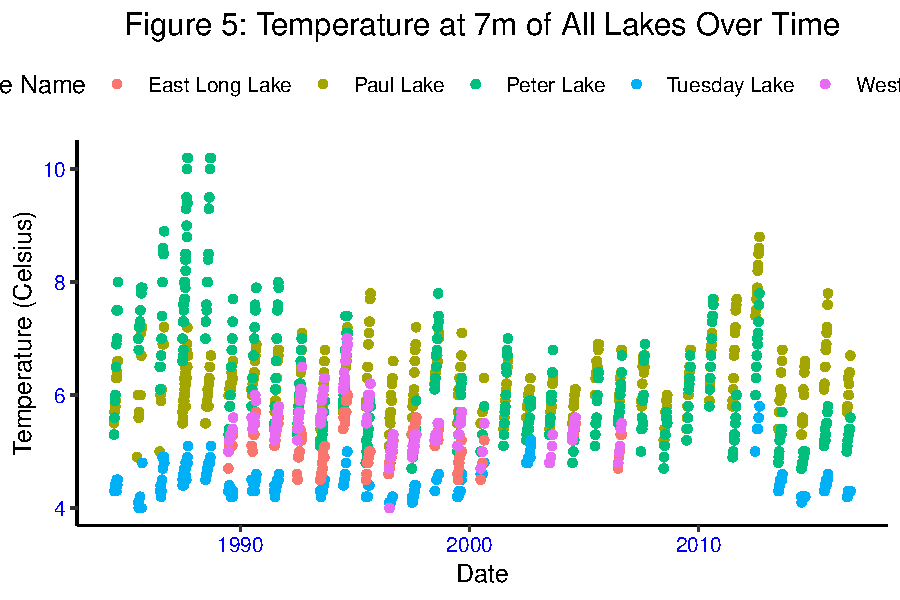
\includegraphics{KBollt_ENV872_FinalProject_files/figure-latex/visualization5-1.pdf}

Likewise, observe in Figure 6: ``Dissolved Oxygen at 7m of All Lakes
Over Time'' that it is difficult to make out a dissolved oxygen trend in
the combined dataset.

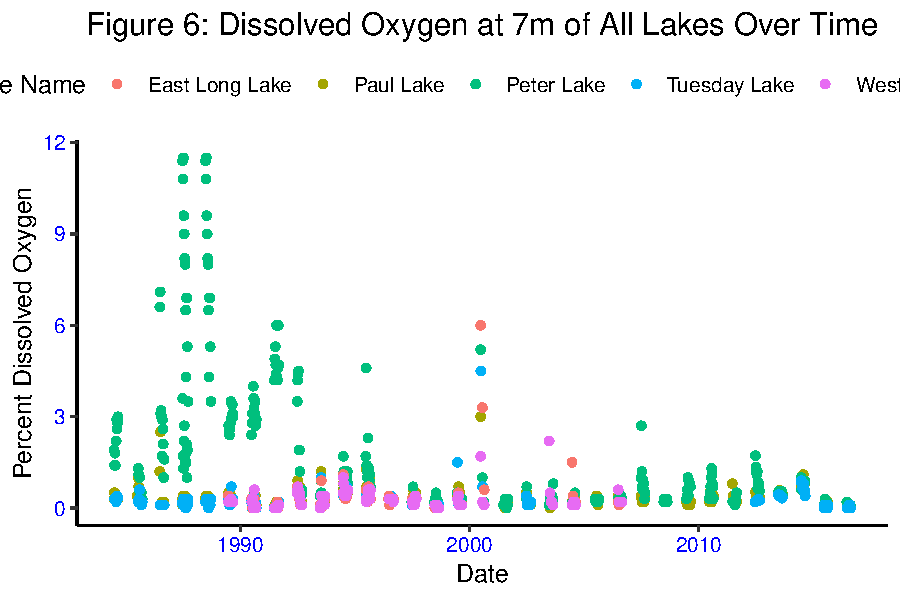
\includegraphics{KBollt_ENV872_FinalProject_files/figure-latex/visualization6-1.pdf}
While we have rejected the null hypothesis that there is a significant
linear trend between the five lakes for either temperature or dissolved
oxygen, we can still look at trends in the individual lakes. In order to
do this, a seasonal Mann-Kendall test is appropriate. I will run 10
seasonal Mann Kendall tests (five lakes and two parameters per lake). I
will set each year's summer as its own season.

\begin{Shaded}
\begin{Highlighting}[]
\CommentTok{#Paul Lake}
\KeywordTok{length}\NormalTok{(}\KeywordTok{unique}\NormalTok{(Paullake_processed}\OperatorTok{$}\NormalTok{year4)) }
\CommentTok{#Tells me how many summers are in the dataset.}
\NormalTok{Paullaketemp_ts <-}\StringTok{ }\KeywordTok{ts}\NormalTok{(Paullake_processed}\OperatorTok{$}\NormalTok{temperature_C,}
                      \DataTypeTok{start =} \KeywordTok{c}\NormalTok{(}\DecValTok{1984}\NormalTok{), }\DataTypeTok{frequency =} \DecValTok{33}\NormalTok{)}
\NormalTok{Paullaketemp_ts}
\NormalTok{Paul_temp_smk <-}\StringTok{ }\KeywordTok{smk.test}\NormalTok{(Paullaketemp_ts)}
\NormalTok{Paul_temp_smk}
\KeywordTok{summary}\NormalTok{(Paul_temp_smk) }
\CommentTok{#The seasonal Mann Kendall test for temperature at Paul Lake had an }
\CommentTok{#overall z-score of 2.2304, an overall p-value of 0.02572 and an }
\CommentTok{#overall S value of 159. This test shows a significant positive }
\CommentTok{#temperature trend over time at Paul Lake.}

\NormalTok{Paullakeo2_ts <-}\StringTok{ }\KeywordTok{ts}\NormalTok{(Paullake_processed}\OperatorTok{$}\NormalTok{dissolvedOxygen,}
                      \DataTypeTok{start =} \KeywordTok{c}\NormalTok{(}\DecValTok{1984}\NormalTok{), }\DataTypeTok{frequency =} \DecValTok{33}\NormalTok{)}
\NormalTok{Paullakeo2_ts}
\NormalTok{Paul_o2_smk <-}\StringTok{ }\KeywordTok{smk.test}\NormalTok{(Paullakeo2_ts)}
\NormalTok{Paul_o2_smk}
\KeywordTok{summary}\NormalTok{(Paul_o2_smk) }\CommentTok{#The seasonal Mann Kendall test for dissolved oxygen}
\CommentTok{#at Paul Lake had an overall z-score of -0.434, an overall p-value of 0.66 }
\CommentTok{#and an overall S value of -31. This test shows a nonsignificant negative}
\CommentTok{#dissolved oxygen trend over time at Paul Lake.}

\CommentTok{#Peter Lake}
\KeywordTok{length}\NormalTok{(}\KeywordTok{unique}\NormalTok{(Peterlake_processed}\OperatorTok{$}\NormalTok{year4)) }
\CommentTok{#Tells me how many summers are in the dataset.}
\NormalTok{Peterlaketemp_ts <-}\StringTok{ }\KeywordTok{ts}\NormalTok{(Peterlake_processed}\OperatorTok{$}\NormalTok{temperature_C,}
                      \DataTypeTok{start =} \KeywordTok{c}\NormalTok{(}\DecValTok{1984}\NormalTok{), }\DataTypeTok{frequency =} \DecValTok{33}\NormalTok{)}
\NormalTok{Peterlaketemp_ts}
\NormalTok{Peter_temp_smk <-}\StringTok{ }\KeywordTok{smk.test}\NormalTok{(Peterlaketemp_ts)}
\NormalTok{Peter_temp_smk}
\KeywordTok{summary}\NormalTok{(Peter_temp_smk) }\CommentTok{#The seasonal Mann Kendall test for temperature }
\CommentTok{#at Peter Lake had an overall z-score of -9.637, an overall p-value of }
\CommentTok{#<2.2x10^-16 and an overall S value of -676. This test shows a significant }
\CommentTok{#negative temperature trend over time at Peter Lake.}

\NormalTok{Peterlakeo2_ts <-}\StringTok{ }\KeywordTok{ts}\NormalTok{(Peterlake_processed}\OperatorTok{$}\NormalTok{dissolvedOxygen,}
                      \DataTypeTok{start =} \KeywordTok{c}\NormalTok{(}\DecValTok{1984}\NormalTok{), }\DataTypeTok{frequency =} \DecValTok{33}\NormalTok{)}
\NormalTok{Peterlakeo2_ts}
\NormalTok{Peter_o2_smk <-}\StringTok{ }\KeywordTok{smk.test}\NormalTok{(Peterlakeo2_ts)}
\NormalTok{Peter_o2_smk}
\KeywordTok{summary}\NormalTok{(Peter_o2_smk) }\CommentTok{#The seasonal Mann Kendall test for dissolved oxygen }
\CommentTok{#at Peter Lake had an overall z-score of -10.557, an overall p-value of }
\CommentTok{#<2.2x10^-16 and an overall S value of -738. This test shows a significant }
\CommentTok{#negative dissolved oxygen trend over time at Peter Lake.}

\CommentTok{#Tuesday Lake}
\KeywordTok{unique}\NormalTok{(Tuesdaylake_processed}\OperatorTok{$}\NormalTok{year4) }\CommentTok{# There are too many gaps in the data, }
\CommentTok{#including a 10 year gap from 2002 to 2012 (which is 30% of the length of }
\CommentTok{#the timeseries), for me to interpolate the whole dataset for purposes of }
\CommentTok{#analysis. I will look at 1984 to 1991, the longest set of continous }
\CommentTok{#data collection.}
\NormalTok{Tuesday_smk <-}\StringTok{ }\NormalTok{Tuesdaylake_processed }\OperatorTok
\StringTok{  }\KeywordTok{filter}\NormalTok{(year4 }\OperatorTok{>=}\StringTok{ }\DecValTok{1984}\NormalTok{, year4 }\OperatorTok{<=}\StringTok{ }\DecValTok{1991}\NormalTok{)}
\NormalTok{Tuesdaylaketemp_ts <-}\StringTok{ }\KeywordTok{ts}\NormalTok{(Tuesday_smk}\OperatorTok{$}\NormalTok{temperature_C,}
                      \DataTypeTok{start =} \KeywordTok{c}\NormalTok{(}\DecValTok{1984}\NormalTok{), }\DataTypeTok{frequency =} \DecValTok{8}\NormalTok{)}
\NormalTok{Tuesdaylaketemp_ts}
\NormalTok{Tuesday_temp_smk <-}\StringTok{ }\KeywordTok{smk.test}\NormalTok{(Tuesdaylaketemp_ts)}
\NormalTok{Tuesday_temp_smk}
\KeywordTok{summary}\NormalTok{(Tuesday_temp_smk) }\CommentTok{#The seasonal Mann Kendall test for temperature at }
\CommentTok{#Tuesday Lake had an overall z-score of -0.56, an overall p-value of 0.57 and }
\CommentTok{#an overall S value of -23. This test shows a nonsignificant negative }
\CommentTok{#temperature trend over time at Tuesday Lake.}

\NormalTok{Tuesdaylakeo2_ts <-}\StringTok{ }\KeywordTok{ts}\NormalTok{(Tuesday_smk}\OperatorTok{$}\NormalTok{dissolvedOxygen,}
                      \DataTypeTok{start =} \KeywordTok{c}\NormalTok{(}\DecValTok{1984}\NormalTok{), }\DataTypeTok{frequency =} \DecValTok{8}\NormalTok{)}
\NormalTok{Tuesdaylakeo2_ts}
\NormalTok{Tuesday_o2_smk <-}\StringTok{ }\KeywordTok{smk.test}\NormalTok{(Tuesdaylakeo2_ts)}
\NormalTok{Tuesday_o2_smk}
\KeywordTok{summary}\NormalTok{(Tuesday_o2_smk) }\CommentTok{#The seasonal Mann Kendall test for dissolved}
\CommentTok{#oxygen at Tuesday Lake had an overall z-score of -3.39, an overall }
\CommentTok{#p-value of 0.0007 and an overall S value of -128. This test shows a }
\CommentTok{#significant negative dissolved oxygen trend over time at Tuesday Lake.}

\CommentTok{#East Long Lake}
\KeywordTok{unique}\NormalTok{(Eastlonglake_processed}\OperatorTok{$}\NormalTok{year4) }\CommentTok{#There are too many gaps in the data, }
\CommentTok{#including no data after 2006 (which is 30% of the length of the timeseries),}
\CommentTok{#for me to interpolate the whole dataset for purposes of analysis. I will }
\CommentTok{#look at 1989 to 2000, the longest set of continous data collection.}
\NormalTok{Eastlong_smk <-}\StringTok{ }\NormalTok{Eastlonglake_processed }\OperatorTok
\StringTok{  }\KeywordTok{filter}\NormalTok{(year4 }\OperatorTok{>=}\StringTok{ }\DecValTok{1989}\NormalTok{, year4 }\OperatorTok{<=}\StringTok{ }\DecValTok{2000}\NormalTok{)}
\NormalTok{Eastlonglaketemp_ts <-}\StringTok{ }\KeywordTok{ts}\NormalTok{(Eastlong_smk}\OperatorTok{$}\NormalTok{temperature_C,}
                      \DataTypeTok{start =} \KeywordTok{c}\NormalTok{(}\DecValTok{1989}\NormalTok{), }\DataTypeTok{frequency =} \DecValTok{12}\NormalTok{)}
\NormalTok{Eastlonglaketemp_ts}
\NormalTok{Eastlong_temp_smk <-}\StringTok{ }\KeywordTok{smk.test}\NormalTok{(Eastlonglaketemp_ts)}
\NormalTok{Eastlong_temp_smk}
\KeywordTok{summary}\NormalTok{(Eastlong_temp_smk) }\CommentTok{#The seasonal Mann Kendall test for temperature }
\CommentTok{#at East Long Lake had an overall z-score of -0.84, an overall p-value }
\CommentTok{#of 0.40 and an overall S value of -32. This test shows a nonsignificant }
\CommentTok{#negative temperature trend over time at East Long Lake.}

\NormalTok{Eastlonglakeo2_ts <-}\StringTok{ }\KeywordTok{ts}\NormalTok{(Eastlong_smk}\OperatorTok{$}\NormalTok{dissolvedOxygen,}
                      \DataTypeTok{start =} \KeywordTok{c}\NormalTok{(}\DecValTok{1989}\NormalTok{), }\DataTypeTok{frequency =} \DecValTok{12}\NormalTok{)}
\NormalTok{Eastlonglakeo2_ts}
\NormalTok{Eastlong_o2_smk <-}\StringTok{ }\KeywordTok{smk.test}\NormalTok{(Eastlonglakeo2_ts)}
\NormalTok{Eastlong_o2_smk}
\KeywordTok{summary}\NormalTok{(Eastlong_o2_smk) }\CommentTok{#The seasonal Mann Kendall test for dissolved }
\CommentTok{#oxygen at East Long Lake had an overall z-score of 0.83, an overall }
\CommentTok{#p-value of 0.41 and an overall S value of 31. This test shows a }
\CommentTok{#nonsignificant positive dissolved oxygen trend over time at East Long Lake.}

\CommentTok{#West Long Lake}
\KeywordTok{unique}\NormalTok{(Westlonglake_processed}\OperatorTok{$}\NormalTok{year4) }\CommentTok{#There are too many gaps in the data, }
\CommentTok{#including no data after 2006 (which is 30% of the length of the timeseries), }
\CommentTok{#for me to interpolate the whole dataset for purposes of analysis. I will }
\CommentTok{#look at 1989 to 2000, the longest set of continous data collection.}
\NormalTok{Westlong_smk <-}\StringTok{ }\NormalTok{Westlonglake_processed }\OperatorTok
\StringTok{  }\KeywordTok{filter}\NormalTok{(year4 }\OperatorTok{>=}\StringTok{ }\DecValTok{1989}\NormalTok{, year4 }\OperatorTok{<=}\StringTok{ }\DecValTok{2000}\NormalTok{)}
\NormalTok{Westlonglaketemp_ts <-}\StringTok{ }\KeywordTok{ts}\NormalTok{(Westlong_smk}\OperatorTok{$}\NormalTok{temperature_C,}
                      \DataTypeTok{start =} \KeywordTok{c}\NormalTok{(}\DecValTok{1989}\NormalTok{), }\DataTypeTok{frequency =} \DecValTok{12}\NormalTok{)}
\NormalTok{Westlonglaketemp_ts}
\NormalTok{Westlong_temp_smk <-}\StringTok{ }\KeywordTok{smk.test}\NormalTok{(Westlonglaketemp_ts)}
\NormalTok{Westlong_temp_smk}
\KeywordTok{summary}\NormalTok{(Westlong_temp_smk) }\CommentTok{#The seasonal Mann Kendall test for temperature }
\CommentTok{#at West Long Lake had an overall z-score of -1.65, an overall p-value of}
\CommentTok{#0.10 and an overall S value of -62. This test shows a nonsignificant }
\CommentTok{#negative temperature trend over time at West Long Lake.}

\NormalTok{Westlonglakeo2_ts <-}\StringTok{ }\KeywordTok{ts}\NormalTok{(Westlong_smk}\OperatorTok{$}\NormalTok{dissolvedOxygen,}
                      \DataTypeTok{start =} \KeywordTok{c}\NormalTok{(}\DecValTok{1989}\NormalTok{), }\DataTypeTok{frequency =} \DecValTok{12}\NormalTok{)}
\NormalTok{Westlonglakeo2_ts}
\NormalTok{Westlong_o2_smk <-}\StringTok{ }\KeywordTok{smk.test}\NormalTok{(Westlonglakeo2_ts)}
\NormalTok{Westlong_o2_smk}
\KeywordTok{summary}\NormalTok{(Westlong_o2_smk) }\CommentTok{#The seasonal Mann Kendall test for dissolved }
\CommentTok{#oxygen at West Long Lake had an overall z-score of -0.47, an overall }
\CommentTok{#p-value of 0.64 and an overall S value of -18. This test shows a}
\CommentTok{#nonsignificant negative dissolved oxygen trend over time at West Long Lake.}
\end{Highlighting}
\end{Shaded}

My data does not appear to be showing a significant change in the
thermocline of any of the five individual lakes, as defined by both
higher temperatures and lower oxygen levels at 7 meters depth. The
results of these tests are summarized in the table below.

Table 3: Summary of Seasonal Mann Kendall results

\begin{longtable}[]{@{}llll@{}}
\toprule
\begin{minipage}[b]{0.14\columnwidth}\raggedright\strut
test run\strut
\end{minipage} & \begin{minipage}[b]{0.22\columnwidth}\raggedright\strut
variable measured\strut
\end{minipage} & \begin{minipage}[b]{0.14\columnwidth}\raggedright\strut
trend\strut
\end{minipage} & \begin{minipage}[b]{0.23\columnwidth}\raggedright\strut
significance of trend\strut
\end{minipage}\tabularnewline
\midrule
\endhead
\begin{minipage}[t]{0.14\columnwidth}\raggedright\strut
seasonal Mann Kendall on Paul Lake\strut
\end{minipage} & \begin{minipage}[t]{0.22\columnwidth}\raggedright\strut
temperature\strut
\end{minipage} & \begin{minipage}[t]{0.14\columnwidth}\raggedright\strut
positive\strut
\end{minipage} & \begin{minipage}[t]{0.23\columnwidth}\raggedright\strut
significant\strut
\end{minipage}\tabularnewline
\begin{minipage}[t]{0.14\columnwidth}\raggedright\strut
seasonal Mann Kendall on Paul Lake\strut
\end{minipage} & \begin{minipage}[t]{0.22\columnwidth}\raggedright\strut
dissolved oxygen\strut
\end{minipage} & \begin{minipage}[t]{0.14\columnwidth}\raggedright\strut
negative\strut
\end{minipage} & \begin{minipage}[t]{0.23\columnwidth}\raggedright\strut
nonsignificant\strut
\end{minipage}\tabularnewline
\begin{minipage}[t]{0.14\columnwidth}\raggedright\strut
seasonal Mann Kendall on Peter Lake\strut
\end{minipage} & \begin{minipage}[t]{0.22\columnwidth}\raggedright\strut
temperature\strut
\end{minipage} & \begin{minipage}[t]{0.14\columnwidth}\raggedright\strut
negative\strut
\end{minipage} & \begin{minipage}[t]{0.23\columnwidth}\raggedright\strut
significant\strut
\end{minipage}\tabularnewline
\begin{minipage}[t]{0.14\columnwidth}\raggedright\strut
seasonal Mann Kendall on Peter Lake\strut
\end{minipage} & \begin{minipage}[t]{0.22\columnwidth}\raggedright\strut
dissolved oxygen\strut
\end{minipage} & \begin{minipage}[t]{0.14\columnwidth}\raggedright\strut
negative\strut
\end{minipage} & \begin{minipage}[t]{0.23\columnwidth}\raggedright\strut
significant\strut
\end{minipage}\tabularnewline
\begin{minipage}[t]{0.14\columnwidth}\raggedright\strut
seasonal Mann Kendall on Tuesday Lake\strut
\end{minipage} & \begin{minipage}[t]{0.22\columnwidth}\raggedright\strut
temperature\strut
\end{minipage} & \begin{minipage}[t]{0.14\columnwidth}\raggedright\strut
negative\strut
\end{minipage} & \begin{minipage}[t]{0.23\columnwidth}\raggedright\strut
nonsignificant\strut
\end{minipage}\tabularnewline
\begin{minipage}[t]{0.14\columnwidth}\raggedright\strut
seasonal Mann Kendall on Tuesday Lake\strut
\end{minipage} & \begin{minipage}[t]{0.22\columnwidth}\raggedright\strut
dissolved oxygen\strut
\end{minipage} & \begin{minipage}[t]{0.14\columnwidth}\raggedright\strut
negative\strut
\end{minipage} & \begin{minipage}[t]{0.23\columnwidth}\raggedright\strut
significant\strut
\end{minipage}\tabularnewline
\begin{minipage}[t]{0.14\columnwidth}\raggedright\strut
seasonal Mann Kendall on East Long Lake\strut
\end{minipage} & \begin{minipage}[t]{0.22\columnwidth}\raggedright\strut
temperature\strut
\end{minipage} & \begin{minipage}[t]{0.14\columnwidth}\raggedright\strut
negative\strut
\end{minipage} & \begin{minipage}[t]{0.23\columnwidth}\raggedright\strut
nonsignificant\strut
\end{minipage}\tabularnewline
\begin{minipage}[t]{0.14\columnwidth}\raggedright\strut
seasonal Mann Kendall on East Long Lake\strut
\end{minipage} & \begin{minipage}[t]{0.22\columnwidth}\raggedright\strut
dissolved oxygen\strut
\end{minipage} & \begin{minipage}[t]{0.14\columnwidth}\raggedright\strut
positive\strut
\end{minipage} & \begin{minipage}[t]{0.23\columnwidth}\raggedright\strut
significant\strut
\end{minipage}\tabularnewline
\begin{minipage}[t]{0.14\columnwidth}\raggedright\strut
seasonal Mann Kendall on West Long Lake\strut
\end{minipage} & \begin{minipage}[t]{0.22\columnwidth}\raggedright\strut
temperature\strut
\end{minipage} & \begin{minipage}[t]{0.14\columnwidth}\raggedright\strut
negative\strut
\end{minipage} & \begin{minipage}[t]{0.23\columnwidth}\raggedright\strut
nonsignificant\strut
\end{minipage}\tabularnewline
\begin{minipage}[t]{0.14\columnwidth}\raggedright\strut
seasonal Mann Kendall on West Long Lake\strut
\end{minipage} & \begin{minipage}[t]{0.22\columnwidth}\raggedright\strut
dissolved oxygen\strut
\end{minipage} & \begin{minipage}[t]{0.14\columnwidth}\raggedright\strut
negative\strut
\end{minipage} & \begin{minipage}[t]{0.23\columnwidth}\raggedright\strut
nonsignificant\strut
\end{minipage}\tabularnewline
\bottomrule
\end{longtable}

As the above table demonstrates, only two of the ten results (20\%) are
both significant and in the predicted direction (positive temperature
trend or negative dissolved oxygen trend); no one lake has both
conditions met. This suggests that the thermoclines on these lakes are
not moving. Let's visualize the temperature and oxygen over the period
of the ten tests I just ran to see if the naked eye agrees with my
statistical analysis.

See in Figure 7: ``Dissolved Oxygen Over Time in Each Lake'' that the
seasonal Mann Kendall results for the five lakes do not show an overall
dissolved oxygen trend at 7 meters in a particular direction.

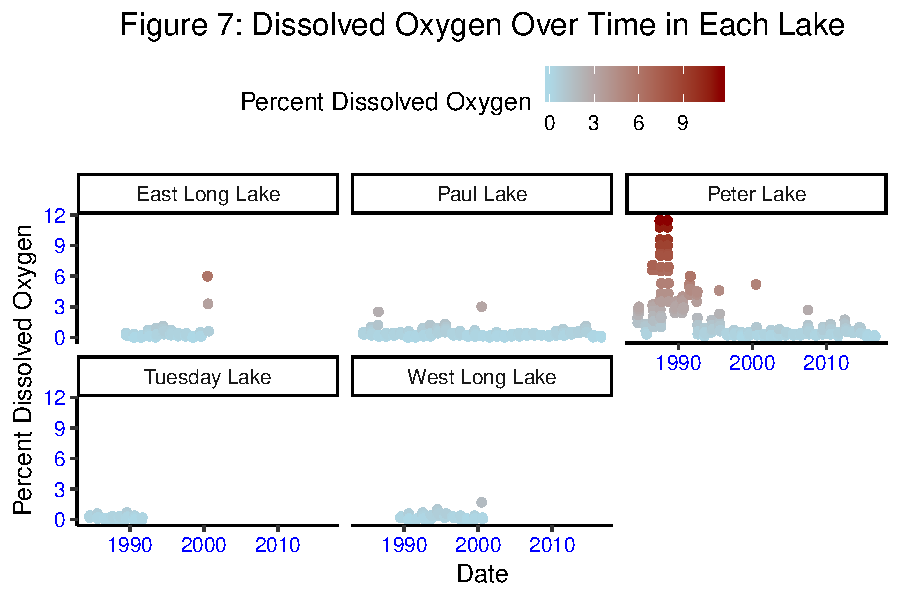
\includegraphics{KBollt_ENV872_FinalProject_files/figure-latex/smk oxygen visualization-1.pdf}

See in Figure 8: ``Temperature Over Time in Each Lake'' that the
seasonal Mann Kendall results for the five lakes do not show an overall
temperature trend at 7 meters in a particular direction.

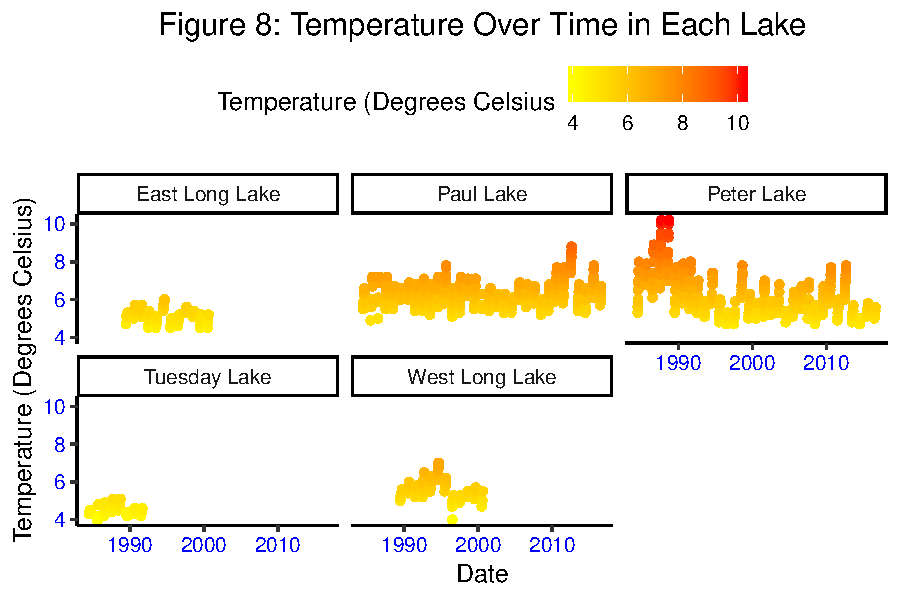
\includegraphics{KBollt_ENV872_FinalProject_files/figure-latex/smk temperature visualization-1.pdf}

\newpage
*

*Discussion** I used repeated measures ANOVA and seasonal Mann Kendall
statistical evaluations of trends in dissolved oxygen and temperature in
five Wisconsin lakes to determine if the thermoclines in these lakes are
moving deeper over time. I found that neither the five lakes in
combination nor any of the five lakes individually are observing both a
significant positive temperature trend and a significant negative
dissolved oxygen trend. The results of my tests seem to run contrary to
the idea that climate change is affecting the water temperatures of the
lakes in this study. However, it may be the case that my tests are
inconclusive by design. I am testing whether the thermocline on these
lakes is moving over time. The location of a lake's thermocline is a
product of water chemistry and physics, especially water density. It may
be the case that the basic physics of water that determine where a
thermocline sets up are not affected by 1 °C of global warming. Perhaps,
given relatively modest warming, it is the relative water density that
determines where the thermocline location sets up. It may be the case
that the steepness and not the location of the thermocline is what is
changing under relatively small amounts of warming. If I were to test
surface water temperature or water temperature at, say, 15 meters, I
would likely see evidence of climate change. It might require larger
levels of warming for the thermocline itself to also move.
Unfortunately, testing this hypothesis is beyond the scope of the
dataset I am analyzing.

\newpage

\textbf{Appendix: Project README File}

\section{badger-thermoclines repository
information}\label{badger-thermoclines-repository-information}

This respository was created as part of a final project for ENVIRON 872
at Duke University. I am looking at NTLR data to determine thermocline
movement on 9 Wisconsin lakes between the period 1984 and 2016. There
are potentially biological ramifications from a shrinking coldwater
summer refuge for organisms such as trout if in fact thermoclines are
setting up at lower levels.

\subsection{Summary}\label{summary}

The dataset used for this project was prepared for Environmental Data
Analytics (ENV 872L) at Duke University's Nicholas School of the
Environment for the spring 2019 semester by Kateri Salk.

The dataset contains physical and chemical data from nine lakes in
Wisconsin. The data was collected between 1984 and 2016 as part of the
NSF-funded North Temperate Lakes Long Term Ecological Research Station.

\subsection{Database Information}\label{database-information}

To find out more information on the North Temperate Lakes Long Term
Ecological Research Station, visit
\url{https://lter.limnology.wisc.edu/about/overview}

The following tool was used to acquire the NTLER data for this project:
(\url{https://lter.limnology.wisc.edu/data})

At the above link, the following data selections were made: * Cascade
Project at North Temperate Lakes LTER Core Data Physical and Chemical
Limnology 1984 - 2016 * Download All Data (csv)

Data was accessed on December 6, 2018.

\subsubsection{Physical and chemical
limnology}\label{physical-and-chemical-limnology}

The data is measured at a station in the middle of each of the nine
lakes. Generally, the data was collected in the morning. The data is
taken at increments, and most data is taken at or below ten meters
depth. The temporal resolution varies across lakes. Some lakes only have
a few years of data, while others have ample data from most or all
years. The data was taken during periods of no ice on the lake. This
means that there is little data during the winter months. While there
are several different measurements taken at these lakes, the two
variables that the thermocline study focuses on are dissolved oxygen and
temperature.

Data collection techniques used during the period 1984-1990 were
described by Carpenter and Kitchell (1993) and data collection
techniques for 1991-1997 were described by Carpenter et al. (2001).

Carpenter, S.R. and J.F. Kitchell (eds.). 1993. The Trophic Cascade in
Lakes. Cambridge University Press, Cambridge, England.

Carpenter, S.R., J.J. Cole, J.R. Hodgson, J.F. Kitchell, M.L. Pace,D.
Bade, K.L. Cottingham, T.E. Essington, J.N. Houser and D.E. Schindler.
2001. Trophic cascades, nutrients and lake productivity: whole-lake
experiments. Ecological Monographs 71: 163-186."

\subsection{Additional Information and
Support}\label{additional-information-and-support}

For more information, please contact the data analyser, \textbf{Keith
Bollt} at
\href{mailto:keith.bollt@duke.edu}{\nolinkurl{keith.bollt@duke.edu}}


\end{document}
